\documentclass[journal]{IEEEtran}
% \documentclass[12pt,letterpaper]{article}
\usepackage[margin=1in]{geometry}
\usepackage[english]{babel}
\usepackage[utf8x]{inputenc}
\usepackage{amsmath}
\usepackage{amssymb} 
% \usepackage[retainorgcmds]{IEEEtrantools}
\usepackage{graphicx}
\usepackage{tabularx}
\usepackage{kpfonts}    % for nice fonts
\usepackage{microtype} 
\usepackage{booktabs}   % for nice tables
\usepackage{bm}         % for bold math
\usepackage{listings}   % for inserting code
\usepackage{verbatim}   % useful for program listings
\usepackage{color} 
\usepackage[colorlinks=true]{hyperref}
% use for hypertext
% \usepackage[colorinlistoftodos]{todonotes}
\usepackage{natbib}

\usepackage{xcolor}
\usepackage{subcaption}

\newtheorem{definition}{Definition}
\newtheorem{theorem}{Theorem}
\newtheorem{proposition}{Proposition}
\newtheorem{corollary}{Corollary}
\newtheorem{lemma}{Lemma}
\newtheorem{example}{Example}

\usepackage{lipsum}

\begin{document}

\title{Hub--Bridge Duality in Social and Communication Networks:\\ A Comparative Centrality and Community Analysis of Twitter, Enron, and Facebook}
        
    \author{
    \IEEEauthorblockN{Author 1},
    \IEEEauthorblockA{\textit{Department of [YOUR DEPARTMENT]} \\
    \textit{UC San Diego}\\
    mail1@mail.com}

    \and
    
    \IEEEauthorblockN{Author 2},
    \IEEEauthorblockA{\textit{Department of [YOUR DEPARTMENT]} \\
    \textit{UC San Diego}\\
    mail2@mail.com}
    \and
    
    \IEEEauthorblockN{Author 3},
    \IEEEauthorblockA{\textit{Department of [YOUR DEPARTMENT]} \\
    \textit{UC San Diego}\\
    mail3@mail.com}
    }
    
\maketitle
%-Title
%+Abstract
\begin{abstract}
We present a comparative structural analysis of five real-world networks
drawn from three public datasets: the Higgs Twitter corpus (retweet,
mention, and reply networks surrounding the 2012 Higgs boson
announcement), the Enron corporate email archive, and the Facebook
ego-network dataset. For each network we compute in-degree, out-degree,
betweenness, and eigenvector centrality, and apply Louvain community
detection. A recurring finding is what we term \textit{hub--bridge
duality}: the highest-degree nodes, which attract the most interactions,
are structurally distinct from the highest-betweenness nodes that mediate
information flow between communities. In the Higgs data, a single
account dominates in-degree and eigenvector centrality across all three
interaction types, yet a different node consistently leads in
betweenness. Top-10\% metric intersection analysis confirms that passive
popularity and active brokerage are largely non-overlapping roles. In the
Enron network, community structure mirrors organizational hierarchy, with
executive inboxes serving as dense intra-community hubs. The Facebook
ego-network yields 16 well-separated communities consistent with
distinct social circles. These results suggest that influence and
connectivity play complementary rather than redundant roles in real-world
networks, with implications for targeted intervention and network
resilience.
\end{abstract}
%-Abstract

\captionsetup{font=footnotesize} % or small


\section{Introduction}

Large-scale social and communication networks encode rich information about
human behavior, influence, and organizational structure.
Understanding how information propagates, who the key actors are, and how
communities form are central questions in network science with applications
ranging from misinformation detection to organizational
auditing~\citep{newman2018networks}.
The rapid growth of online platforms has produced massive interaction graphs
whose structural properties — degree distributions, centrality rankings,
community partitions — offer quantitative proxies for latent social phenomena
such as popularity, brokerage, and group affiliation.

A natural question is whether the most \textit{popular} nodes in a network
are also the most \textit{structurally important}.
High in-degree captures passive popularity: the accounts most mentioned, the
inboxes most emailed.
High betweenness centrality, by contrast, captures brokerage: the nodes
whose removal would most fragment the flow of information between otherwise
distant groups.
Prior work on scale-free networks \citep{barabasi1999} has shown that
degree distributions in real-world graphs are heavy-tailed, implying that
a small number of hubs attract a disproportionate share of connections.
However, degree alone does not determine a node's role as a structural
bridge, and the relationship between these two notions of importance
remains dataset-dependent.

In this paper we investigate this question across three complementary
real-world datasets:
(i)~the \textit{Higgs Twitter dataset} \citep{higgs2013}, which captures
three interaction modalities — retweets, mentions, and replies — surrounding
the announcement of the Higgs boson discovery;
(ii)~the \textit{Enron email corpus}, which provides a longitudinal record
of internal corporate communication at Enron Corporation; and
(iii)~the \textit{Facebook ego-network dataset} \citep{leskovec2012}, which
represents friendship circles of selected users on Facebook.
These datasets span directed event-driven graphs, directed organizational
graphs, and an undirected friendship graph, providing breadth across
network types.

For each network we compute four standard centrality metrics — in-degree,
out-degree, betweenness, and eigenvector centrality — and apply the Louvain
community detection algorithm \citep{blondel2008}.
We introduce a \textit{top-10\% intersection analysis} that quantifies the
pairwise overlap between the highest-ranked nodes under each metric,
revealing which notions of importance coincide and which diverge.
Beyond centrality, we measure clustering coefficients and average
shortest-path lengths, and compare each network against three canonical
null models — Erd\H{o}s--R\'enyi~\citep{erdos1959}, Watts--Strogatz~\citep{watts1998},
and Barab\'asi--Albert~\citep{barabasi1999} — to characterise the
generative regime each network most closely resembles.
We also contrast Louvain with Label Propagation to evaluate the
sensitivity of community structure to algorithm choice.

Our central finding is what we term \textit{hub--bridge duality}: across all
five networks, the highest-degree nodes are largely distinct from the
highest-betweenness nodes, indicating that popularity and brokerage are
complementary rather than redundant structural roles.
In the Higgs data a single account dominates in-degree and eigenvector
centrality across all three interaction types, yet a different node
consistently leads in betweenness.
The Facebook network is unambiguously small-world, with clustering
($\bar{C} = 0.606$) approaching Watts--Strogatz levels and short average
path length ($\ell \approx 3.7$), yet its heavy-tailed degree distribution
matches Barab\'asi--Albert — no single model captures both properties.
In the Enron network, Louvain communities mirror the corporate hierarchy,
with executive inboxes serving as intra-community hubs, and Louvain
consistently achieves higher modularity than Label Propagation across
all networks ($Q = 0.835$ vs.\ $0.737$ on Facebook; $0.628$ vs.\ $0.382$
on Enron).

The remainder of this paper is organized as follows.
Section~\ref{sec:related} goes over a quick summary of relevant related works.
Section~\ref{sec:model} defines the network models and centrality measures.
Section~\ref{sec:data} describes each dataset.
Section~\ref{sec:results} presents our experimental results.
Section~\ref{sec:conclusion} concludes with a discussion of limitations and
future directions.

Our GitHub repo can be found at the following link:
https://github.com/realrusssobti/ece227-course-project/tree/main

\section{Related Work}
\label{sec:related}

The in-depth analysis of complex networks has its foundation in mathematical models. The network analysis works in the early stages were centered more on random graphs proposed by \citet{erdos1959}, and this has been the baseline for understanding edge probability. However, real social and organizational networks are rare. So, \citet{watts1998} introduced the small-world network model to represent high local clustering with remarkably short average path lengths between any two nodes.
Human communication networks consist of email exchanges that exhibit scale-free properties. The work by \citet{barabasi1999} established that as networks grow, nodes connect via "preferential attachment," which leads to the emergence of hubs and a degree distribution that follows a power law. This has been the basis for the analysis of the Enron dataset, Facebook dataset, and Twitter dataset. The works by \citet{newman2018networks} provide a comprehensive theoretical foundation for understanding structural metrics, such as degree centrality and shortest path lengths.
Though the above papers cover macro-level topologies, to understand the internal substructures of a network, we were using the Louvain method. \citet{blondel2008} introduced this model to perform a highly efficient heuristic for modularity optimization. This has helped in unfolding the hidden communities within large datasets.
         
\section{Model}
\label{sec:model}

\subsection{Network Representation}

We model each dataset as a directed graph $G = (V, E)$ where $V$ is the
set of nodes (users or email addresses) and $E \subseteq V \times V$ is the
set of directed edges (interactions).
For the Facebook dataset we use an undirected graph $G = (V, E)$ since
friendship is a symmetric relation.
Edge weights, where present, encode interaction frequency (e.g.\ number
of retweets between a pair of users).

\subsection{Centrality Metrics}

We compute four node-level centrality measures.

\textbf{In-degree centrality.}
For a node $v$, $k^{\text{in}}(v) = |\{u : (u,v) \in E\}|$ counts the number
of incoming edges. In interaction networks, high in-degree corresponds to
nodes that are frequently targeted (e.g.\ popular accounts).

\textbf{Out-degree centrality.}
$k^{\text{out}}(v) = |\{u : (v,u) \in E\}|$ counts outgoing edges and
identifies prolific senders or broadcasters.

\textbf{Betweenness centrality.}
\begin{equation}
    C_B(v) = \sum_{s \neq v \neq t} \frac{\sigma_{st}(v)}{\sigma_{st}}
\end{equation}
where $\sigma_{st}$ is the total number of shortest paths from $s$ to $t$
and $\sigma_{st}(v)$ is the number of those paths that pass through $v$.
Nodes with high betweenness act as \textit{bridges} connecting otherwise
distant parts of the network.

\textbf{Eigenvector centrality.}
The eigenvector centrality vector $\mathbf{x}$ satisfies
$A\mathbf{x} = \lambda_{\max} \mathbf{x}$,
where $A$ is the adjacency matrix and $\lambda_{\max}$ is the largest
eigenvalue. High eigenvector centrality identifies nodes that are connected
to other important nodes, capturing recursive influence.

\subsection{Community Detection}

We apply the \textit{Louvain algorithm} \citep{blondel2008} to detect
communities by iteratively maximizing modularity
\begin{equation}
    Q = \frac{1}{2m} \sum_{ij} \left[ A_{ij} - \frac{k_i k_j}{2m} \right]
        \delta(c_i, c_j),
\end{equation}
where $m = |E|$, $k_i$ is the degree of node $i$, and $\delta(c_i, c_j) = 1$
iff nodes $i$ and $j$ are in the same community.
For directed networks (Higgs, Enron) we convert to an undirected graph
prior to community detection.

\subsection{Graph-Level Properties}

Beyond node-level centrality, we measure two graph-level structural
properties~\citep{newman2018networks}.

\textbf{Clustering coefficient.}
The local clustering coefficient of node $v$ is
\begin{equation}
    c(v) = \frac{|\{(u,w) \in E : u,w \in \mathcal{N}(v)\}|}{k(v)(k(v)-1)},
\end{equation}
where $\mathcal{N}(v)$ is the set of neighbours of $v$ and $k(v) = |\mathcal{N}(v)|$.
The network average $\bar{C} = \frac{1}{|V|}\sum_v c(v)$ quantifies the
tendency of nodes to form tightly connected triples.
High $\bar{C}$ relative to a random graph is a hallmark of
small-world networks~\citep{watts1998}.

\textbf{Average shortest-path length.}
\begin{equation}
    \ell = \frac{1}{|V|(|V|-1)} \sum_{s \neq t} d(s,t),
\end{equation}
where $d(s,t)$ is the length of the shortest path from $s$ to $t$.
For large networks we estimate $\ell$ via BFS sampling from
500 randomly chosen source nodes in the largest connected component.

\subsection{Top-10\% Intersection Analysis}

To assess agreement between metrics, we compute the pairwise intersection
of nodes appearing in the top 10\% of each centrality ranking.
A large intersection between, say, betweenness and in-degree indicates
that popular nodes also serve as structural bridges;
a small intersection indicates that hubs and bridges are structurally
distinct populations.

\begin{figure*}[ht]
    \centering
    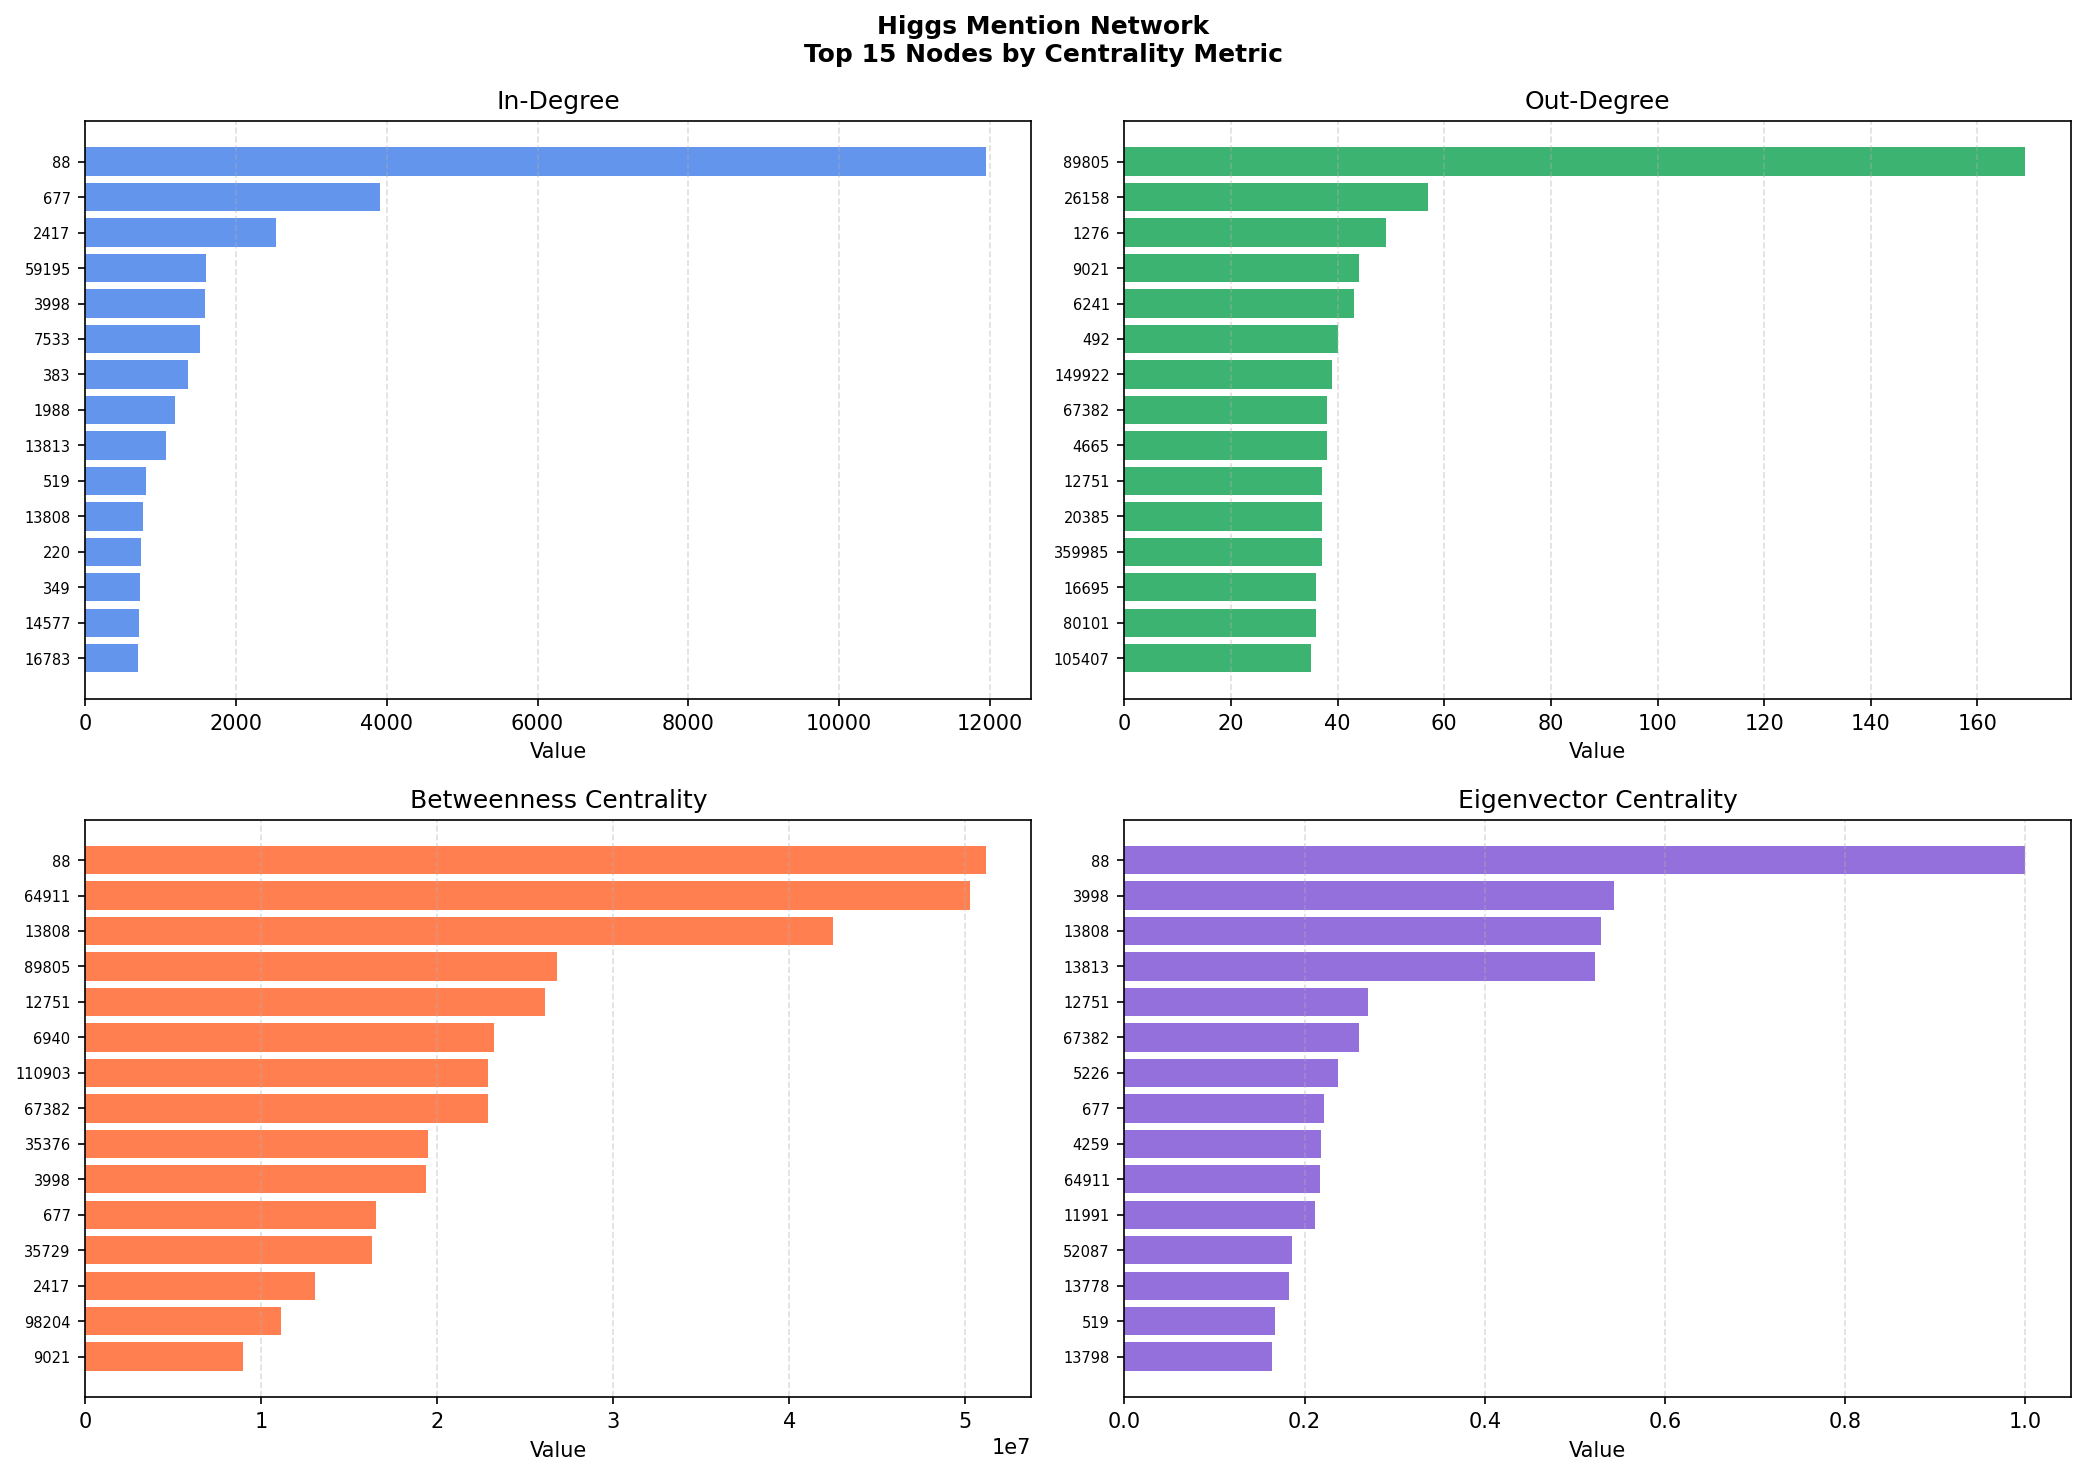
\includegraphics[width=0.95\linewidth]{figures/higgs_mention_centrality.png}
    \caption{Top-15 nodes by each centrality metric in the Higgs Mention network.
             Node \texttt{88} dominates in-degree and eigenvector centrality while
             node \texttt{64911} ranks highest in betweenness, illustrating the
             hub--bridge distinction described in Section~\ref{sec:model}.}
    \label{fig:mention_centrality}
\end{figure*}

\section{Dataset Description}
\label{sec:data}

We study three public datasets that span qualitatively different network
types: a real-time social-media event, a corporate email archive, and a
friendship graph.
Table~\ref{tab:datasets} summarizes the key statistics of each network.

\begin{table}[ht]
\centering
\caption{Dataset statistics. Degree values are for the directed graphs
         (Higgs, Enron) or the undirected graph (Facebook).}
\label{tab:datasets}
\begin{tabular}{lrrrl}
\toprule
\textbf{Network} & \textbf{Nodes} & \textbf{Edges} & \textbf{Avg.\ Degree} & \textbf{Type} \\
\midrule
Higgs Mention  & 116{,}408 & 150{,}818 & 1.30 & Directed \\
Higgs Reply    &  38{,}918 &  32{,}523 & 0.84 & Directed \\
Higgs Retweet  & 256{,}491 & 328{,}132 & 1.28 & Directed \\
Enron Email    &  15{,}597 &  53{,}226 & 3.41 & Directed \\
Facebook       &   4{,}039 &  88{,}234 & 21.8 & Undirected \\
\bottomrule
\end{tabular}
\end{table}

\subsection{Higgs Twitter Dataset}

The Higgs Twitter dataset~\cite{higgs2013} was collected around July 4, 2012,
the day the discovery of the Higgs boson was announced.
It comprises three directed interaction networks derived from Twitter activity:

\begin{itemize}
    \item \textbf{Retweet network} (256{,}491 nodes): directed edge $(u \to v)$
          indicates that user $u$ retweeted a post by $v$.
          This is the largest and densest of the three networks.
    \item \textbf{Mention network} (116{,}408 nodes): directed edge $(u \to v)$
          indicates that user $u$ mentioned $v$ in a tweet.
    \item \textbf{Reply network} (38{,}918 nodes): directed edge $(u \to v)$
          indicates that user $u$ replied directly to a tweet by $v$.
          This is the smallest and most conversational of the three.
\end{itemize}

All three networks exhibit heavy-tailed in-degree distributions consistent
with a power-law, as shown in Figure~\ref{fig:higgs_deg}.

\begin{figure*}[ht]
    \centering
    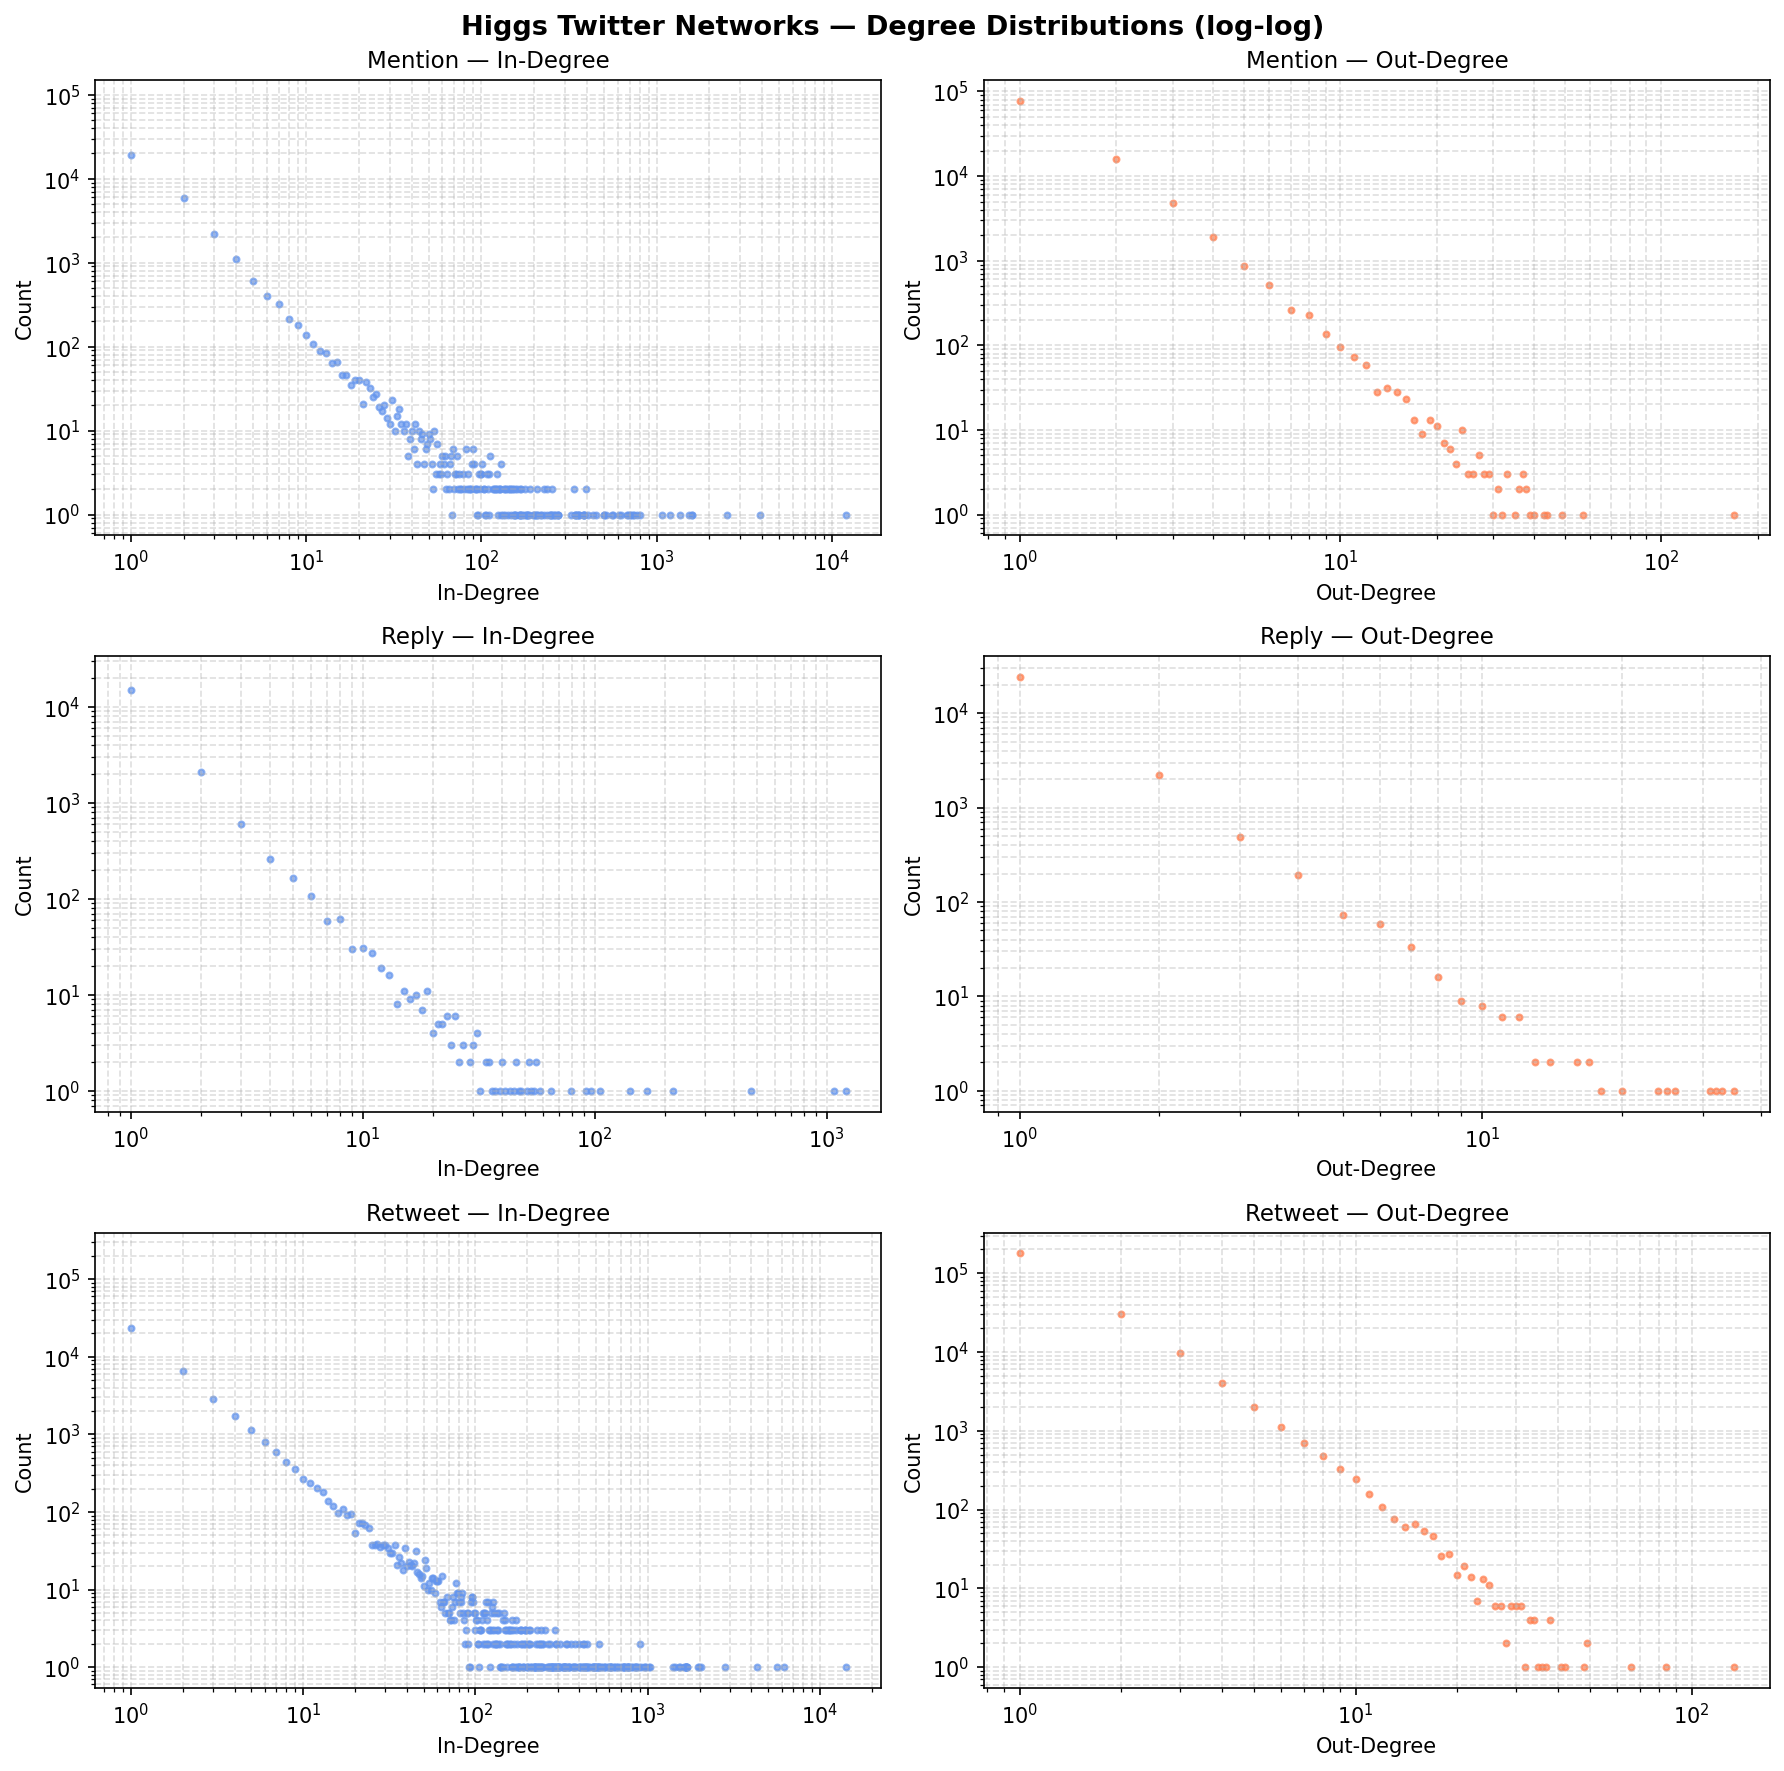
\includegraphics[width=0.85\linewidth]{figures/higgs_all_deg.png}
    \caption{Log-log degree distributions for the three Higgs Twitter networks
             (rows: Mention, Reply, Retweet), showing in-degree (left) and
             out-degree (right).
             All three exhibit heavy-tailed in-degree distributions consistent
             with preferential-attachment dynamics.
             Out-degree distributions are considerably more concentrated,
             indicating that most users participate moderately while a small
             number act as prolific broadcasters.}
    \label{fig:higgs_deg}
\end{figure*}

\subsection{Enron Email Dataset}

The Enron email dataset is derived from the publicly released Enron email
corpus and contains approximately 50{,}000 messages parsed for sender/receiver
pairs.
The resulting directed graph captures communication flow among
15{,}597 unique email addresses with 53{,}226 directed edges.
Figure~\ref{fig:enron_deg} shows the degree distribution of the
undirected projection.

\begin{figure}[!t]
    \centering
    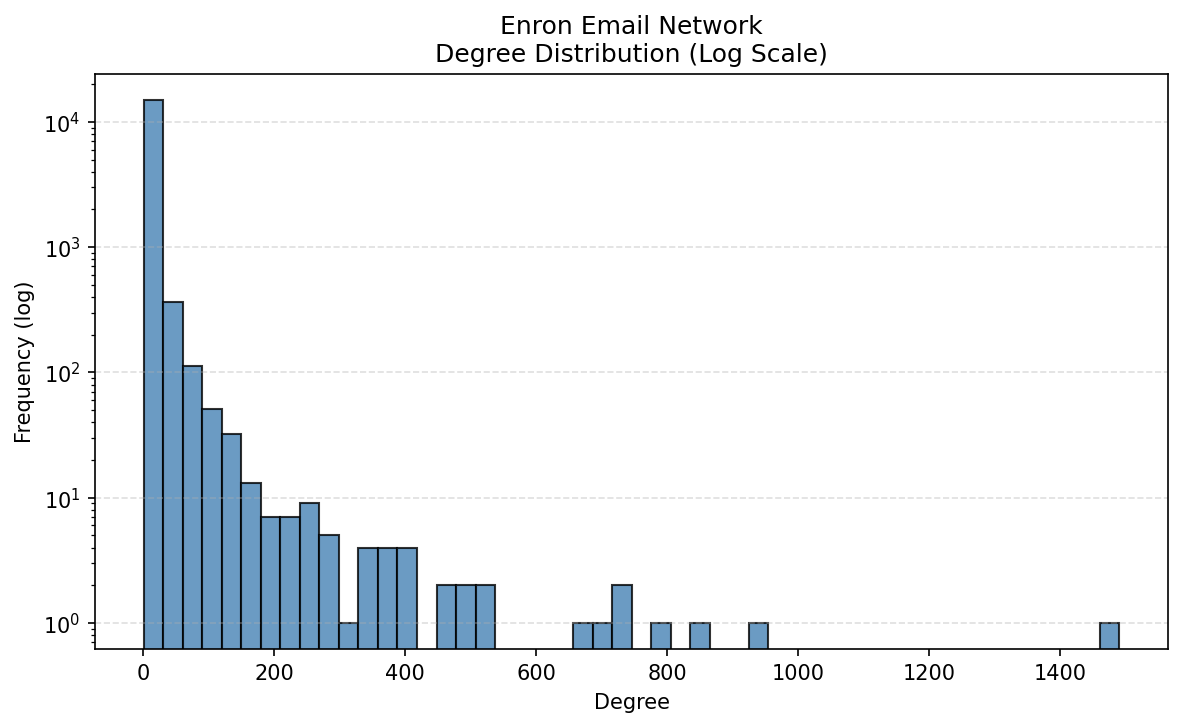
\includegraphics[width=0.9\linewidth]{figures/enron_deg.png}
    \caption{Degree distribution of the Enron email network (undirected
             projection, log scale).
             The distribution is heavy-tailed, with a small number of
             addresses — primarily executive inboxes and distribution lists —
             receiving a disproportionate volume of mail.}
    \label{fig:enron_deg}
\end{figure}

\subsection{Facebook Ego-Network Dataset}

The Facebook combined dataset~\cite{leskovec2012} comprises 4{,}039 nodes
and 88{,}234 undirected edges assembled from the ego-networks of ten
anonymized users.
With an average degree of 21.8, this is by far the densest of our three
datasets, reflecting the tightly clustered nature of real-world friendship
networks.

\section{Results}
\label{sec:results}

\subsection{Centrality Analysis — Higgs Twitter}

Figure~\ref{fig:mention_centrality} (Section~\ref{sec:model}) shows the
top-15 nodes for the Mention network.
A consistent pattern emerges across all three Higgs networks: a single
dominant hub (node \texttt{88}) captures the highest in-degree and
eigenvector centrality, while a structurally distinct bridge node
(node \texttt{64911} in Retweet, \texttt{13808} in Reply) leads in
betweenness centrality.
This \textit{hub--bridge duality} suggests that the most-mentioned accounts
are not necessarily the primary conduits through which information flows
between communities.

Figure~\ref{fig:retweet_centrality} provides the equivalent four-panel view
for the Retweet network, which is the largest and most influential propagation
channel during the Higgs boson event.

\begin{figure*}[!t]
    \centering
    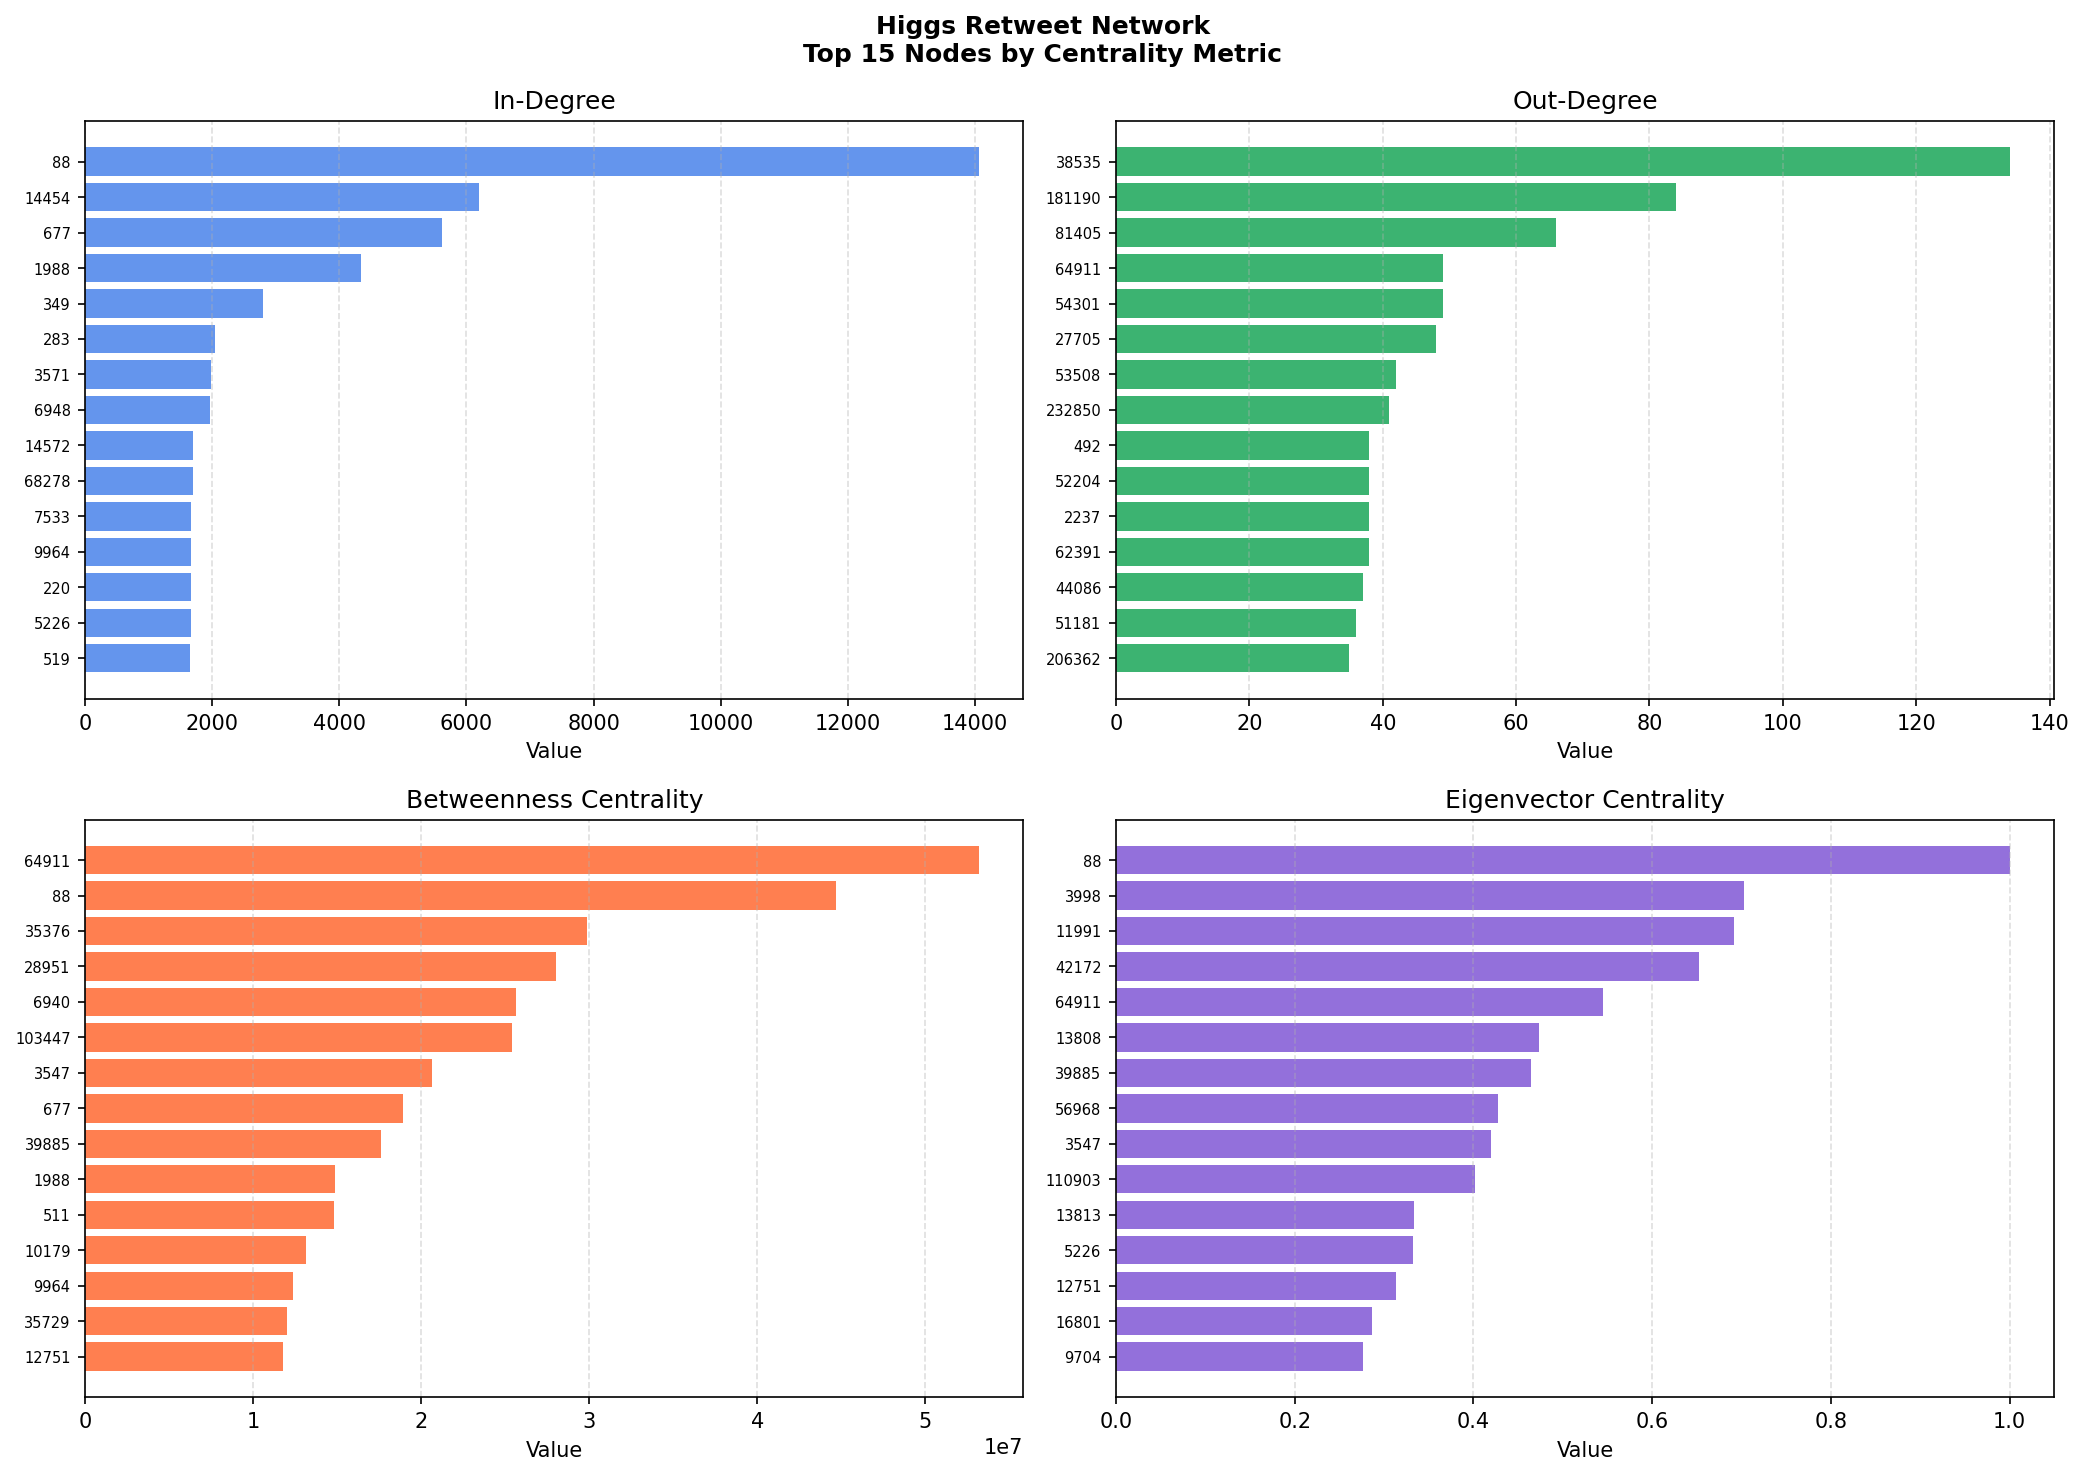
\includegraphics[width=0.95\linewidth]{figures/higgs_retweet_centrality.png}
    \caption{Top-15 nodes by each centrality metric in the Higgs Retweet network.
             Node \texttt{88} dominates in-degree (14{,}060 retweets) while
             \texttt{64911} leads in betweenness, confirming the hub--bridge
             distinction across all Higgs interaction types.}
    \label{fig:retweet_centrality}
\end{figure*}

\subsection{Top-10\% Metric Intersections}

Figure~\ref{fig:intersections} shows pairwise top-10\% intersections for
each network.
Several observations stand out:

\begin{itemize}
    \item \textbf{In-Deg $\cap$ Out-Deg} is the smallest intersection in all
          three networks, confirming that popular recipients generally do not
          also broadcast heavily — passive popularity and active participation
          are distinct roles.
    \item In the Retweet network, \textbf{Betweenness $\cap$ Eigenvector}
          yields 18{,}628 nodes — the largest pairwise intersection of any
          metric pair across all datasets — indicating that structural bridges
          and influential neighbors are strongly correlated in the retweet graph.
    \item The Reply network shows the tightest intersections overall,
          consistent with its smaller size and more conversational structure.
\end{itemize}

\begin{figure*}[ht]
    \centering
    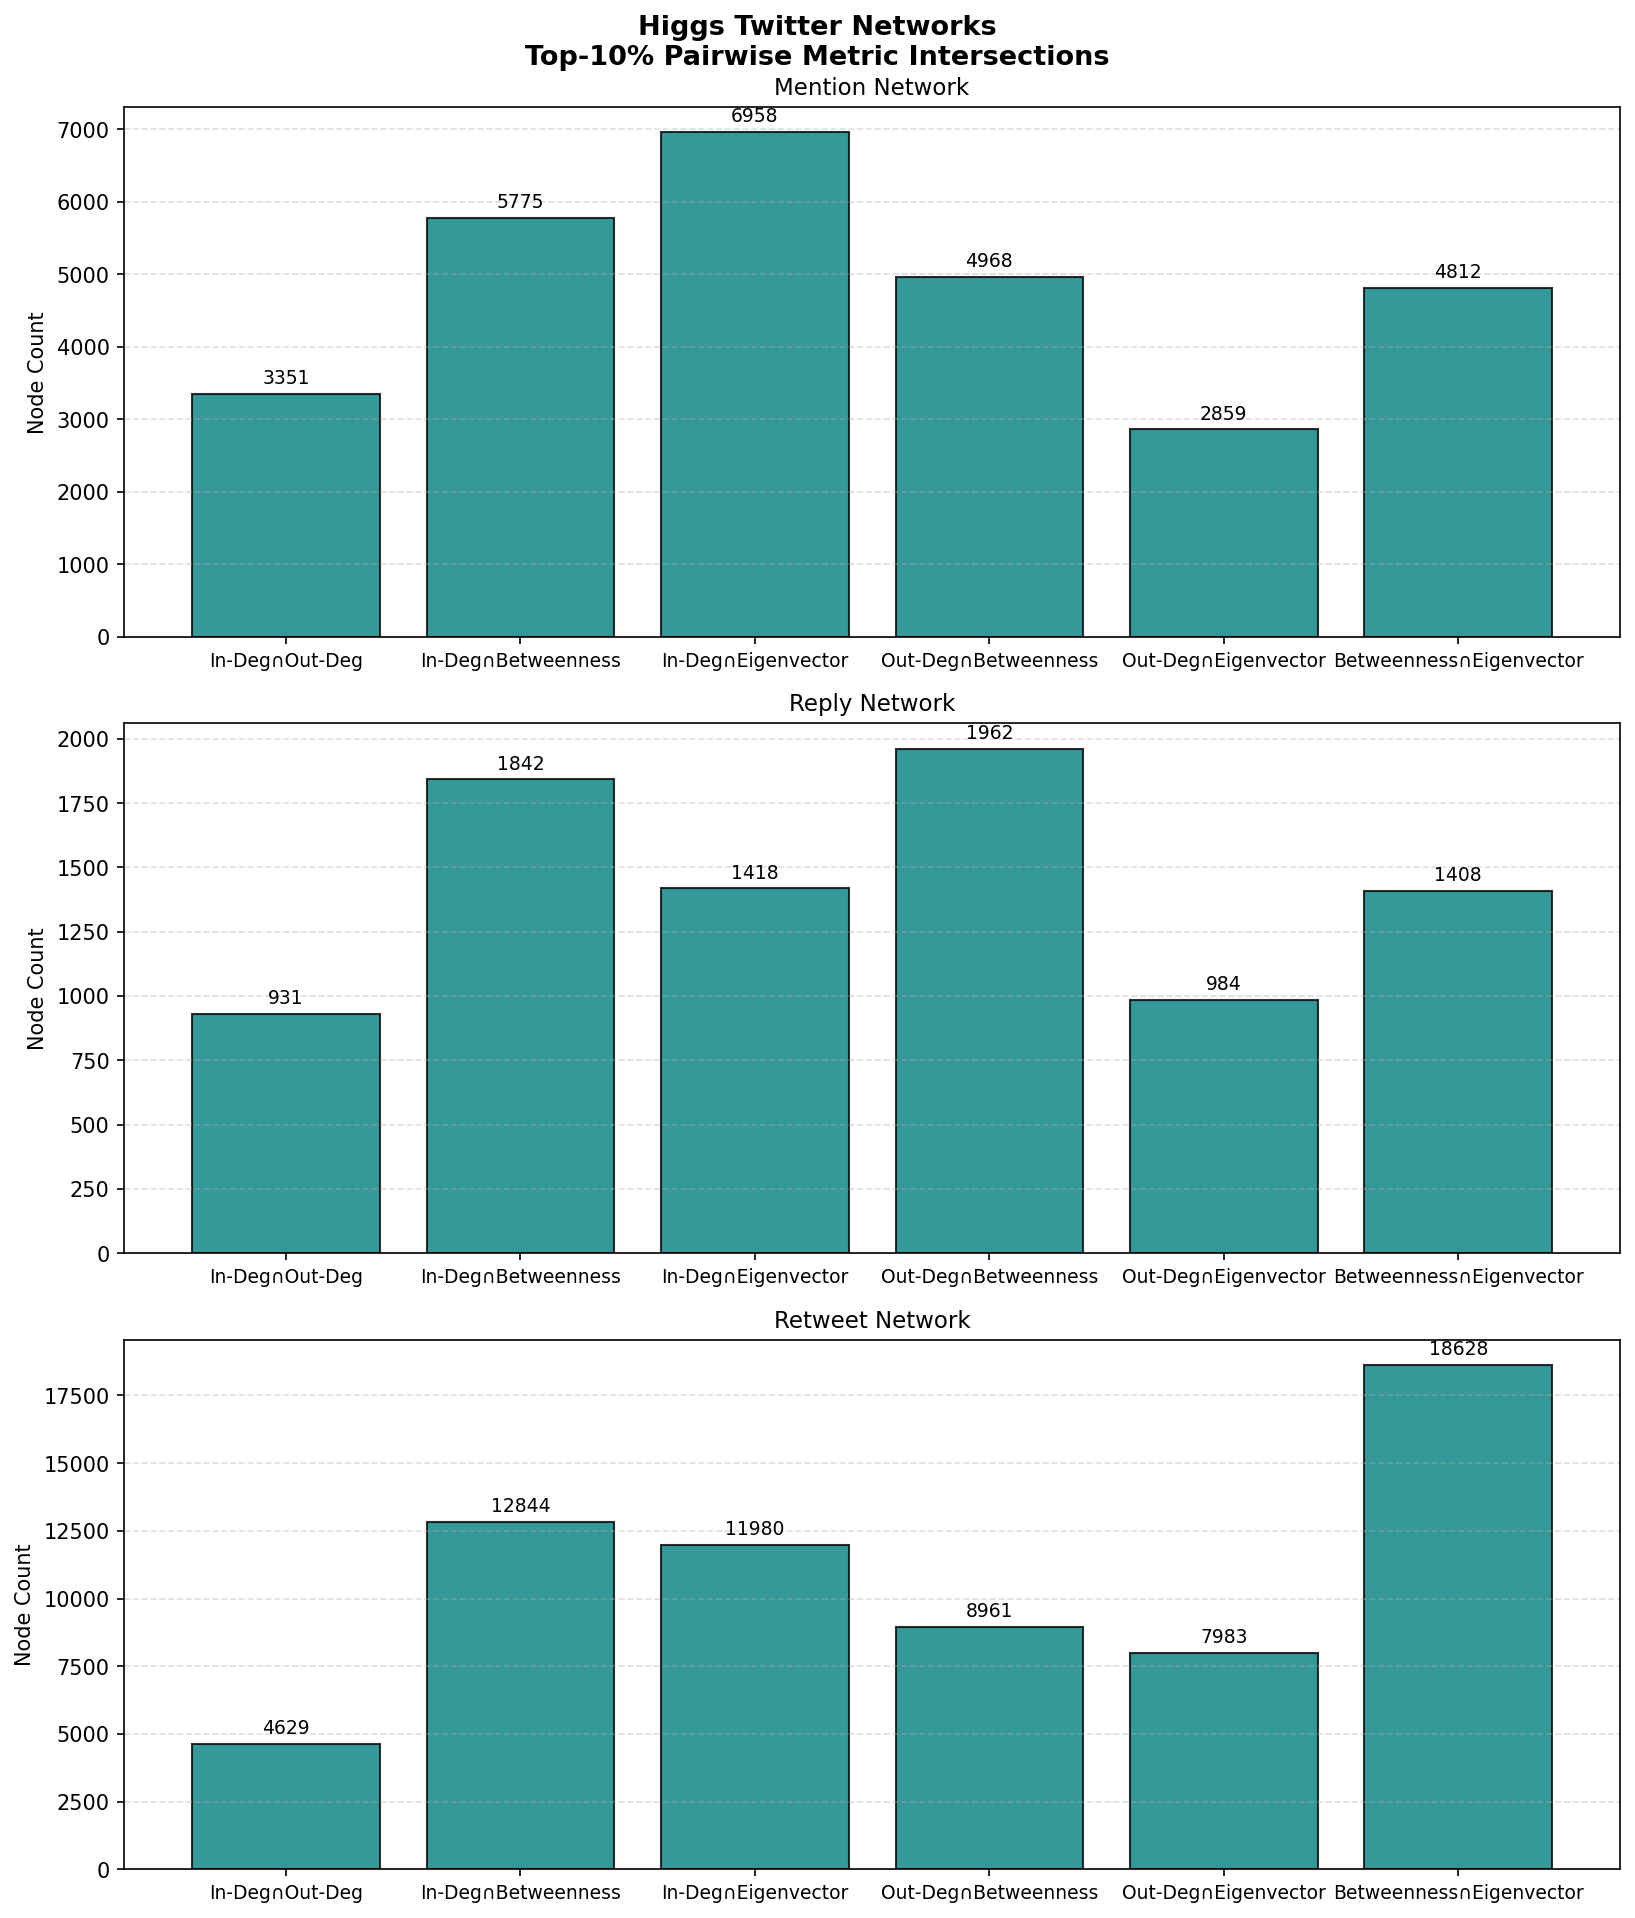
\includegraphics[width=0.78\linewidth]{figures/higgs_all_intersections.png}
    \caption{Top-10\% pairwise metric intersections for the Mention (top),
             Reply (middle), and Retweet (bottom) networks.
             In-Deg $\cap$ Out-Deg is consistently the smallest intersection,
             while Betweenness $\cap$ Eigenvector is the largest in the
             Retweet network.}
    \label{fig:intersections}
\end{figure*}

\subsection{Cross-Network Comparison}

Figure~\ref{fig:comparison} compares node count, edge count, and average
in-degree across the three Higgs networks.
The Retweet network is more than twice as large as the Mention network and
six times the size of the Reply network, reflecting the asymmetric
virality of the Higgs boson announcement.

\begin{figure*}[!t]
    \centering
    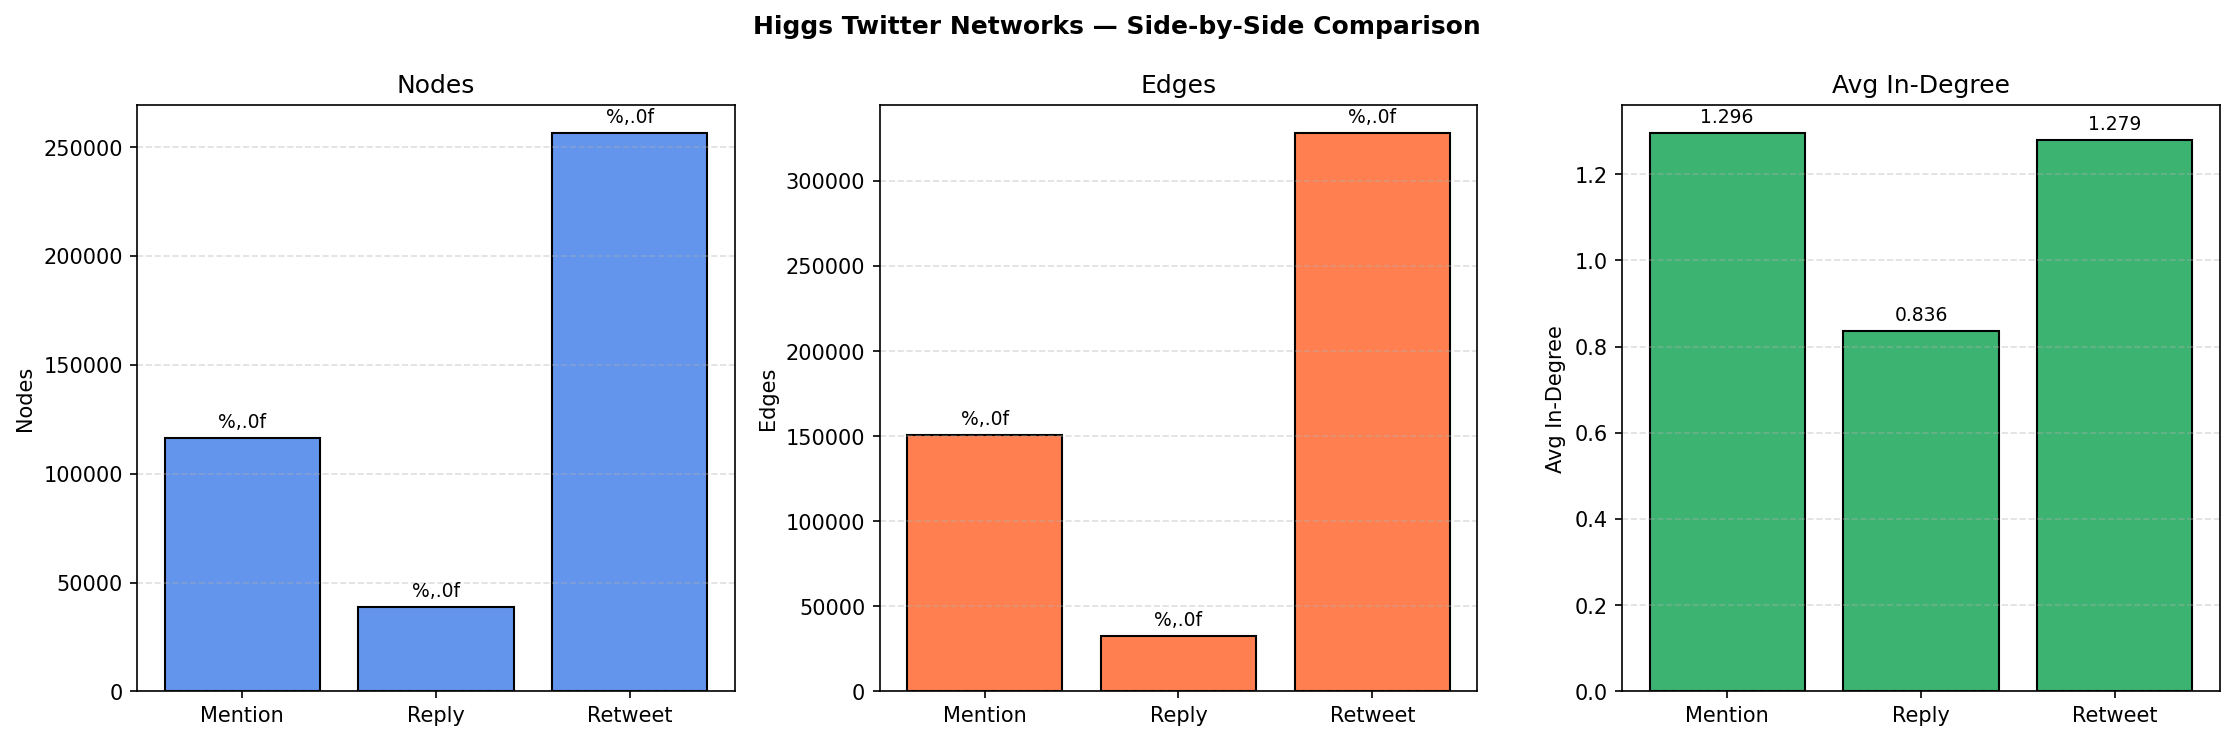
\includegraphics[width=0.48\linewidth]{figures/higgs_comparison.png}
    \hfill
    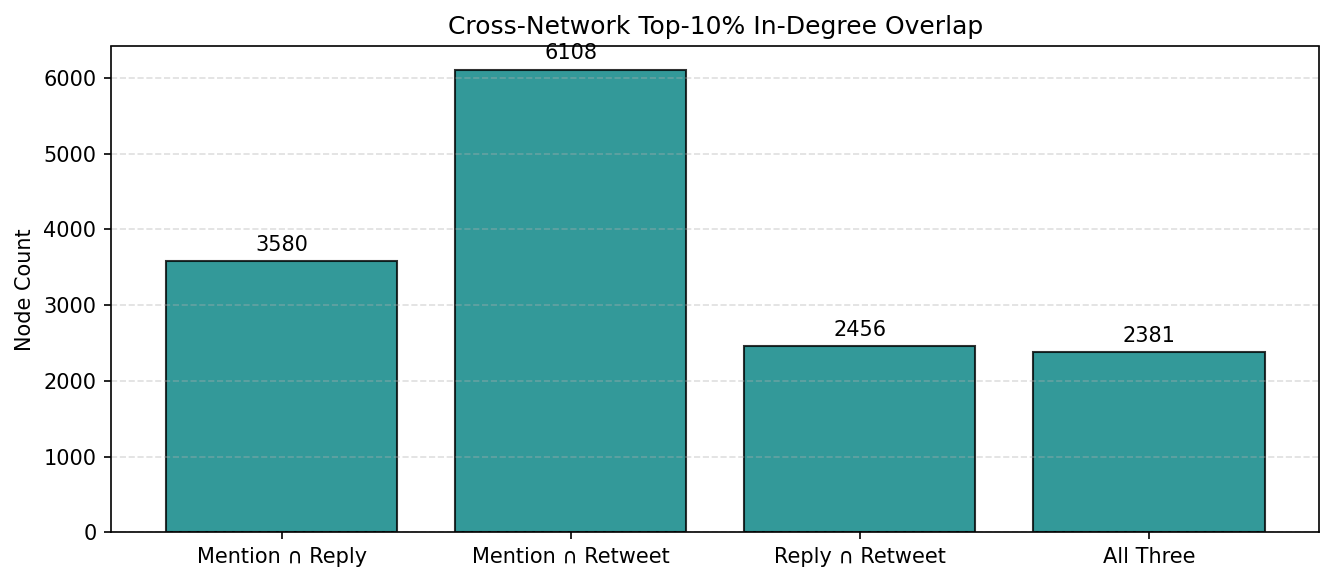
\includegraphics[width=0.48\linewidth]{figures/higgs_overlap.png}
    \caption{\textit{Left}: Side-by-side comparison of the three Higgs Twitter
             networks by number of nodes, edges, and average in-degree.
             \textit{Right}: Cross-network top-10\% in-degree overlap.
             Mention $\cap$ Retweet yields 6,100 shared high-influence users
             — the largest pairwise overlap — while only 2,301 nodes appear
             in the top 10\% across all three networks simultaneously.}
    \label{fig:comparison}
    \label{fig:overlap}
\end{figure*}

Figure~\ref{fig:comparison} (right) shows that 6,100 nodes appear in the
top 10\% by in-degree in both the Mention and Retweet networks — the largest
pairwise overlap — while only 2,301 nodes are consistently influential across
all three interaction types simultaneously.

\subsection{Enron Email Network}

Figure~\ref{fig:enron_centrality} shows the top-15 Enron nodes by each
centrality metric.
\texttt{sally.beck@enron.com} (COO) dominates both in-degree and betweenness,
indicating she was both a primary recipient and a critical communication bridge
across departments.
High out-degree belongs to \texttt{sally.beck} and \texttt{bob.ambrecht},
consistent with executive broadcast behaviour.
Notably, betweenness and eigenvector centrality surface different executives
than in-degree alone — \texttt{don.baughman} ranks highly in betweenness
despite modest in-degree, suggesting a broker role spanning otherwise
disconnected groups.

\begin{figure*}[ht]
    \centering
    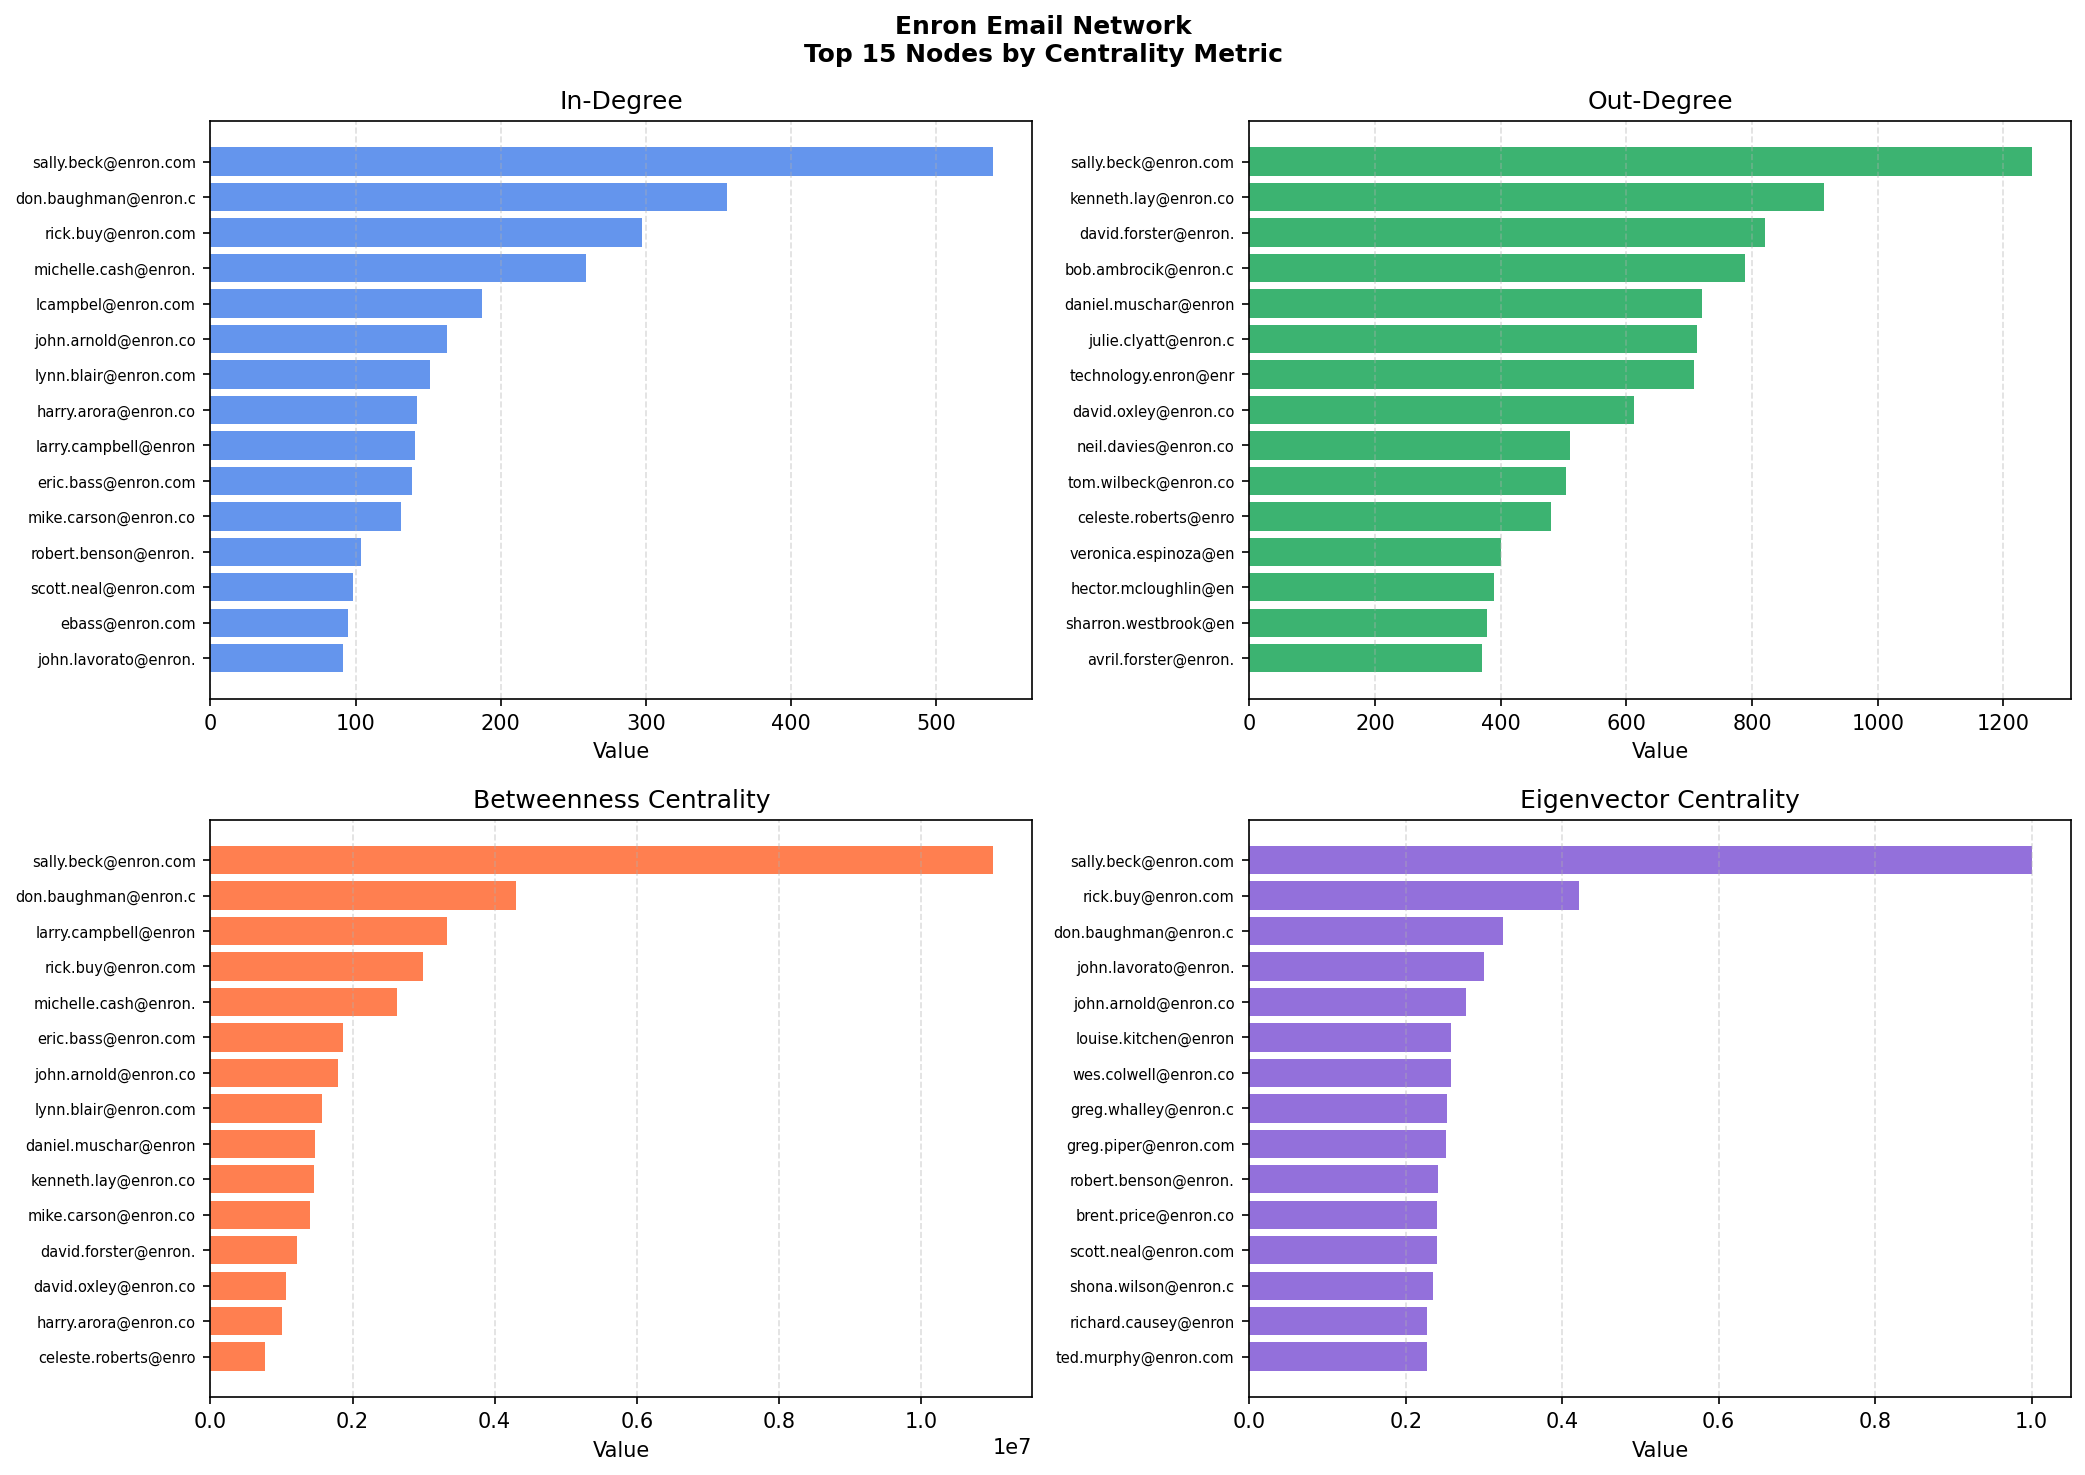
\includegraphics[width=0.95\linewidth]{figures/enron_centrality.png}
    \caption{Top-15 Enron email addresses by centrality metric.
             High in-degree nodes correspond to executive inboxes and
             distribution lists; high betweenness nodes represent
             organizational bridges between departments.}
    \label{fig:enron_centrality}
\end{figure*}

The Louvain algorithm identified 252
communities in the Enron network, as shown in Figure~\ref{fig:enron_comm}.
The distribution of community sizes is highly skewed, with a few large
communities (likely business units) and many small peripheral clusters.
Figure~\ref{fig:enron_exec} provides a richer view of the executive
sub-network, with node size proportional to degree and edge thickness
proportional to email volume.

\begin{figure*}[!t]
    \centering
    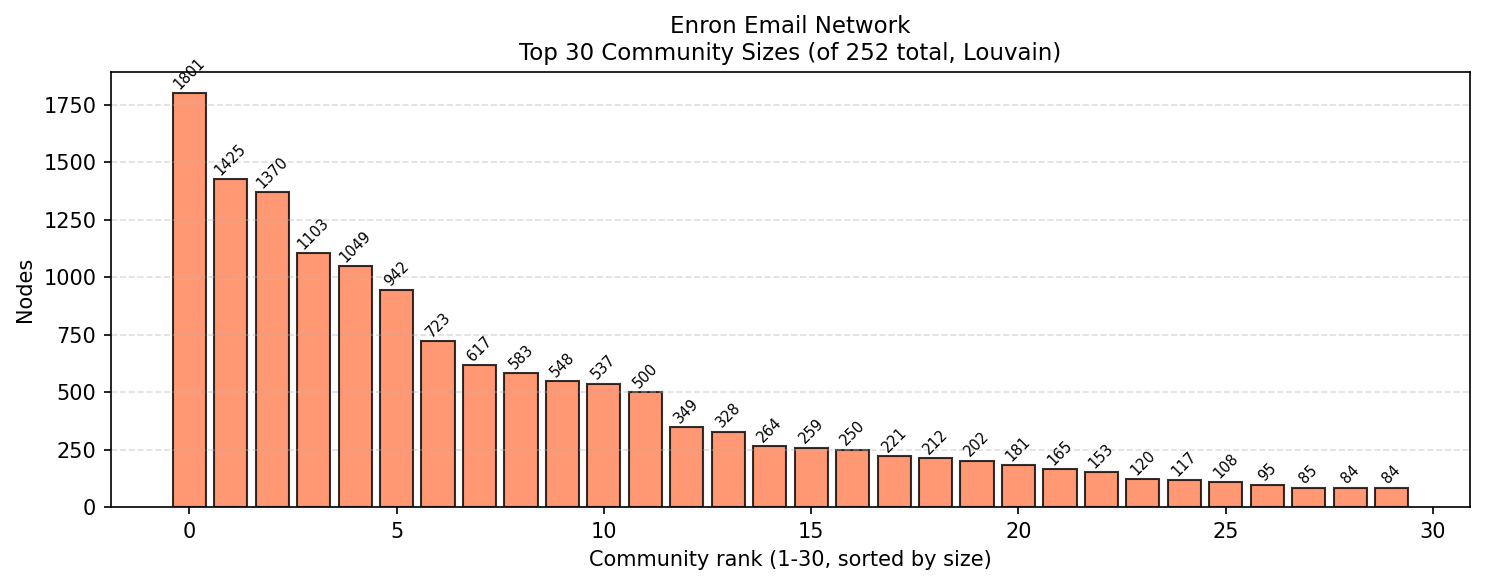
\includegraphics[width=0.55\linewidth]{figures/enron_communities.png}
    \vspace{0.5em}\\
    \includegraphics[width=0.95\linewidth]{figures/enron_exec_network.png}
    \caption{\textit{Top}: Louvain community sizes for the Enron email
             network (top 30 of 252 total), sorted by size. The rapid
             drop-off indicates a few dominant business-unit clusters and
             many small peripheral groups.
             \textit{Bottom}: Executive sub-network showing top senders
             for each VP/CEO. Node size is proportional to degree;
             edge thickness encodes email volume.
             \texttt{sally.beck@enron.com} (COO) is the largest hub.}
    \label{fig:enron_comm}
    \label{fig:enron_exec}
\end{figure*}

\subsection{Facebook Ego-Network}

Figure~\ref{fig:fb_deg} shows the degree distribution and Louvain community
structure of the Facebook network.
The 16 communities range from 19 to 548 nodes and likely correspond to the
distinct social circles of the ten anonymised ego users; the uneven size
distribution reflects the varying social reach of each ego.
In contrast to Enron's 252 fine-grained departmental clusters, Facebook yields
far fewer but larger communities, consistent with the tighter clustering and
higher average degree (21.8) of a friendship graph.

\begin{figure*}[!t]
    \centering
    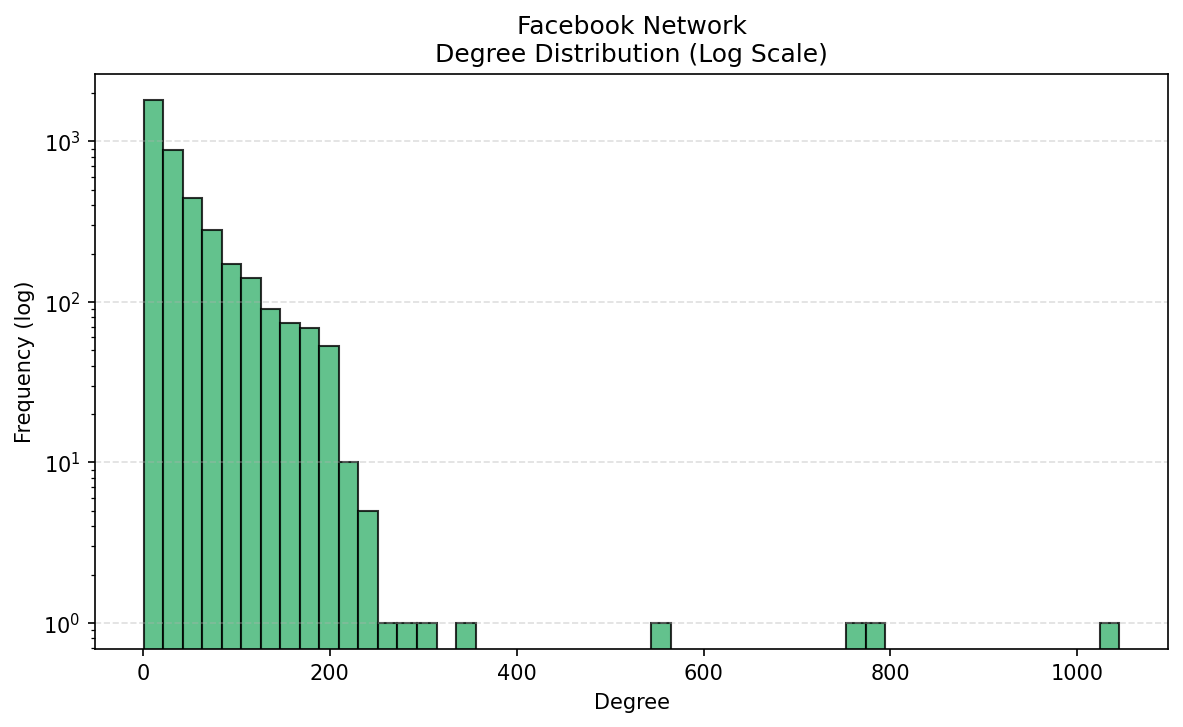
\includegraphics[width=0.48\linewidth]{figures/fb_deg.png}
    \hfill
    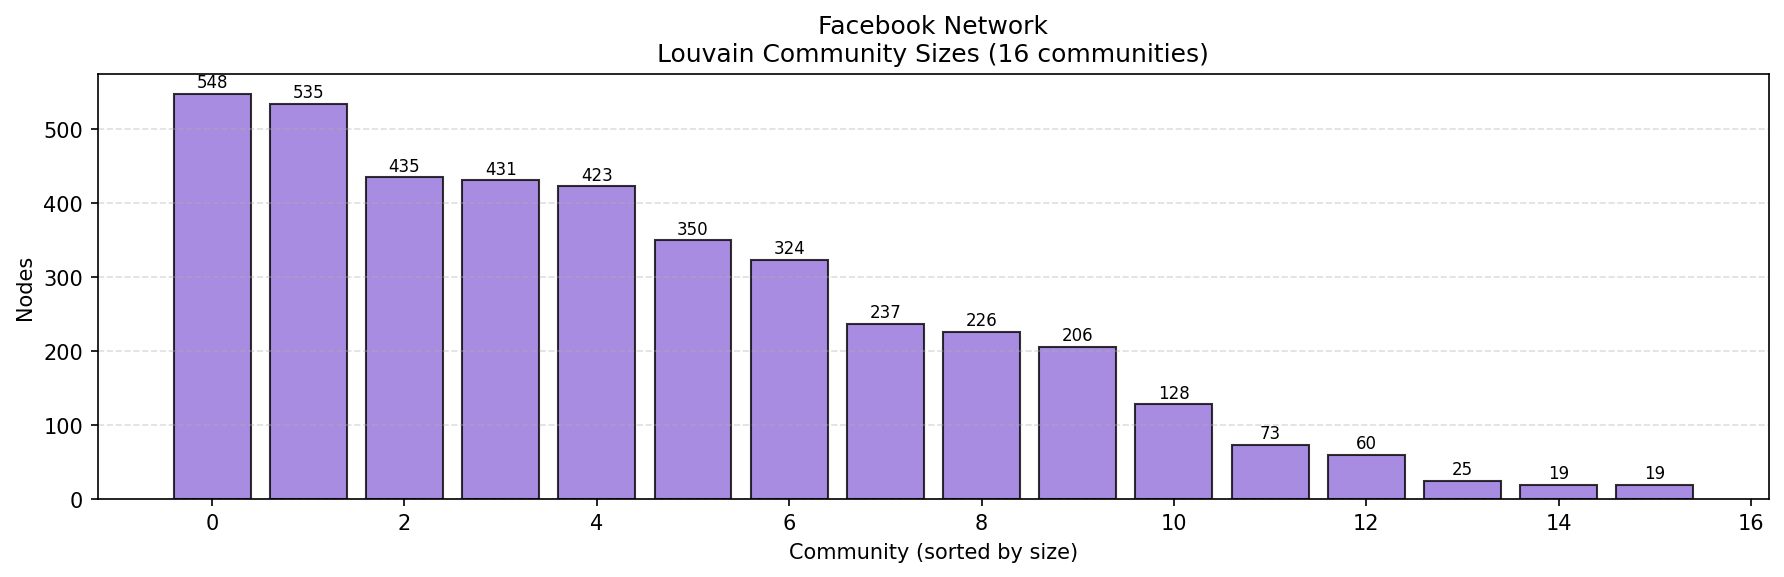
\includegraphics[width=0.48\linewidth]{figures/fb_communities.png}
    \caption{\textit{Left}: Degree distribution of the Facebook combined
             network (log scale). The distribution is heavy-tailed but
             less extreme than the directed Higgs networks, reflecting
             the reciprocal nature of friendship ties.
             \textit{Right}: Louvain community sizes for the Facebook
             network. The 16 communities range from 19 to 548 nodes and
             likely correspond to distinct social circles of the ego users.}
    \label{fig:fb_deg}
    \label{fig:fb_comm}
\end{figure}

\section{Conclusion}
\label{sec:conclusion}

% TODO: Write 1-2 paragraphs summarizing findings.

We analyzed five real-world networks across three datasets using a consistent
pipeline of degree statistics, betweenness centrality, eigenvector centrality,
and Louvain community detection.
A recurring finding is the \textit{hub--bridge duality}: the nodes with the
highest degree (or eigenvector centrality) are not the same nodes that
maximize information flow across the network.
This has practical implications — removing a high-degree node may not
disrupt communication as much as targeting a high-betweenness bridge.

In the Higgs Twitter data, node \texttt{88} dominates in-degree and
eigenvector centrality across all three interaction types, confirming its
role as the primary information source during the Higgs boson event.
In the Enron network, the community structure reflects the underlying
organizational hierarchy, with executive inboxes acting as dense hubs
within their respective communities.
The Facebook ego-network yields 16 well-separated communities consistent
with distinct social circles.

% TODO: Add any quantitative take-aways specific to your paper's thesis.

\section{Future Work}
\label{sec:future}

Several extensions of this work are natural:

\textbf{Temporal analysis.}
The Higgs dataset includes activity timestamps in
\texttt{higgs-activity\_time.txt}.
A natural follow-up is to study how centrality rankings evolve over time and
whether early adopters of the Higgs boson story maintain their influence.

\textbf{Multiplex centrality.}
Because mention, reply, and retweet networks share the same node set, one
could compute \textit{multiplex centrality} measures that aggregate
information across layers, identifying nodes that are simultaneously
important across all interaction types.

\textbf{Robustness and targeted removal.}
Given the hub--bridge distinction, a comparative simulation of random vs.\
targeted node removal (targeting hubs vs.\ bridges) would quantify the
resilience of each network.

\textbf{Feature-based community interpretation.}
The Facebook dataset includes rich node feature vectors (\texttt{node\_to\_features.txt}).
Linking detected communities to demographic or interest features could
validate the semantic meaning of the Louvain partitions.


\clearpage
\bibliographystyle{apalike}
\bibliography{aguiar}

\newpage

\begin{IEEEbiography}[{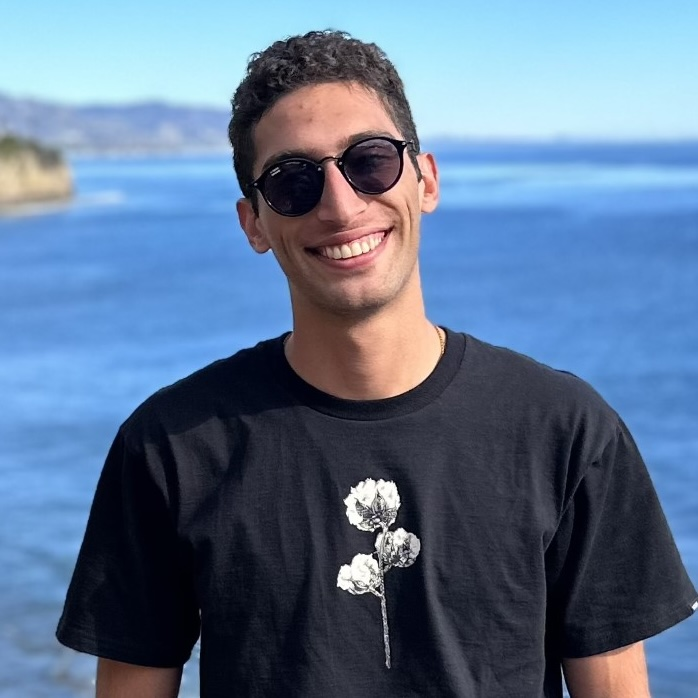
\includegraphics[width=1in,height=1.25in,clip,keepaspectratio]{figures/raman.jpg}}]{Raman Ebrahimi} earned his B.Sc. degrees in Physics and Industrial Engineering from Sharif University of Technology in 2022. His thesis was on the spread of (Dis)Information over the Networks. He received his M.S. degree in March 2025 and his thesis, titled ``From Games to Predictions: Strategic Behavior in Networks and Classification'' focused on applications of game theory and network science in modeling agent behavior. He is now working towards his Ph.D. in Electrical and Computer Engineering at the University of California, San Diego with a special focus on machine learning and data science. His research focuses on game theory, network economics, games on networks, and computational social science. 
\end{IEEEbiography}
\vspace{-1in}
\begin{IEEEbiography}[{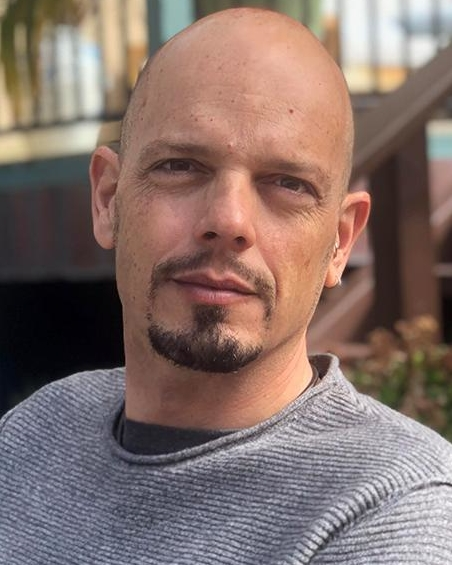
\includegraphics[width=1in,height=1.25in,clip,keepaspectratio]{figures/massimo.jpg}}] {Massimo Franceschetti} graduated in computer engineering from the University of Naples in 1997. He received M.S. and Ph.D. degrees in electrical engineering from the California Institute of Technology in 1999, and 2003 respectively. His doctoral thesis, entitled ``Wireless Networks, from Collective Behavior to the Physics of Propagation'' was awarded the Wilts Prize for best thesis in electrical engineering at Caltech in 2003. He also received the 2000 Walker von Brimer award for outstanding research at Caltech. Franceschetti has held visiting positions at the Vrije Universiteit Amsterdam in the Netherlands, the Ecole Polytechnique Federale de Lausanne in Switzerland, and the University of Trento in Italy. Before joining UCSD, he was a post-doctoral scholar at University of California at Berkeley for two years. 
\end{IEEEbiography}

\end{document}